% Capítulo 6
\chapter{Estudo Experimental}
\label{cap:cap6}

Este capítulo consiste em apresentar o estudo, envolve a concepção de contexto do experimento, das configurações e características dos elementos envolvidos, a seleção das variáveis influenciadoras, o controle e a instrumentação do experimento, sua execução, a captura de dados durante experimentação, e por fim, a análise e conclusões obtidas a partir desses resultados. 

O objetivo do experimento é analisar a viabilidade do uso de mecanismos de \textit{throttling} como candidato para aumentar a disponibilidade dos elementos presentes em \textit{IoT} através do ajuste de comportamento por ação de limiares de atuação que consideram seus aspectos energéticos para assim,  prolongar a autonomia energética dos dispositivos. A abordagem é aderente e cobre os elementos presentes na taxonomia proposta no Capítulo \ref{cap:cap4} permitindo comparação e análise entre dispositivos que diferem sobre o fato de terem sua operação ajustada mediante \textit{throttling} ou não. 

\section{Metodologia}

O experimento pretende comparar os efeitos do mecanismo de \textit{throttling} em dispositivos com capacidade de coleta de energia, com foco em examinar a disponibilidade de cada um relacionada aos aspectos energéticos em condições de capacidade e atuação semelhantes.

\begin{figure}[H]
	\centering
	\caption{Etapas do Estudo Experimental.}
	\label{fig:cap6metodologia}
	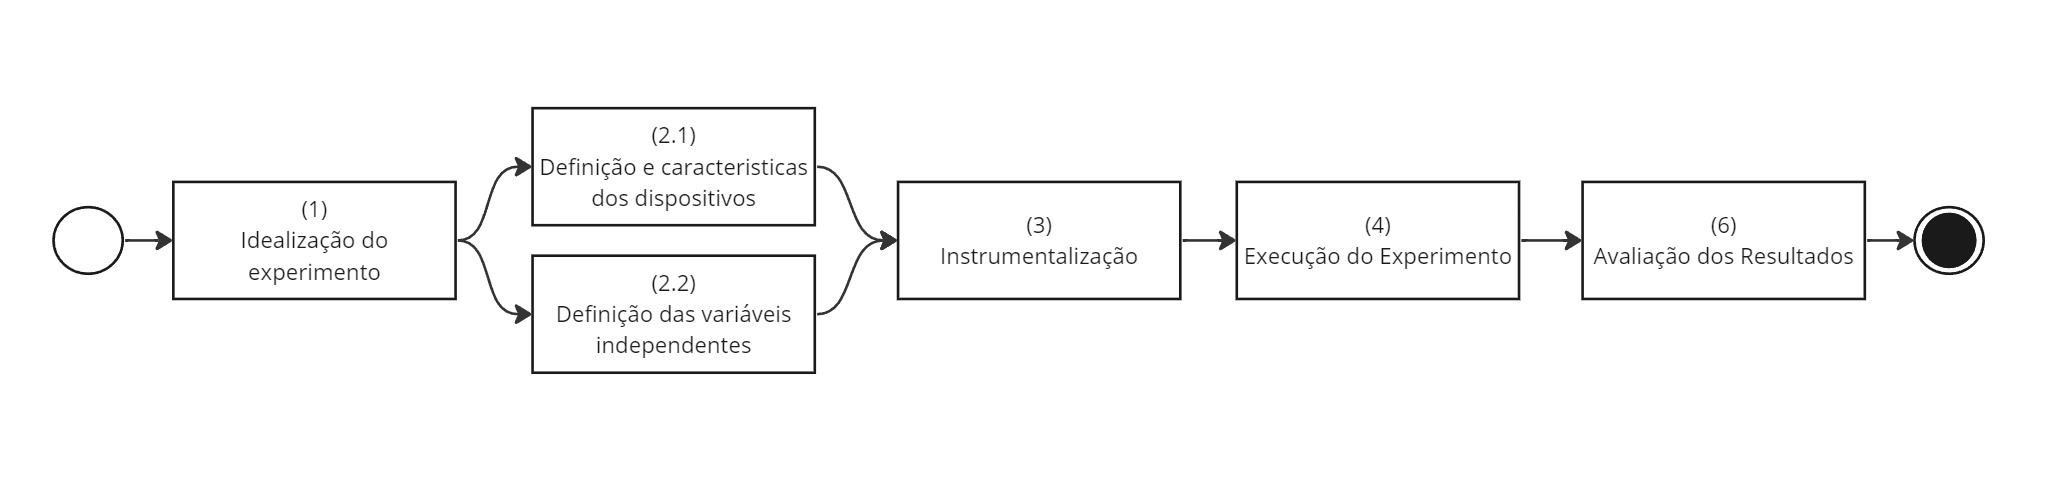
\includegraphics[width=1\linewidth]{Imagens/cap6/cap6metodologia.jpg}
	
	Fonte: elaborado pelo autor.
\end{figure} 

Para tal, buscou-se observar a influência do fator limitante na alteração do comportamento dos participantes em relação aos valores de energia coletada e reserva energética. Além disso, compreender sua eficiência na tomada de decisão em atender ou não às solicitações, em virtude da autoanálise de suas capacidades à medida que a variação de energia disponível ocorre. Este estudo visa analisar o uso de \textit{throttling} como possível solução para estender a disponibilidade de dispositivos com capacidade de coleta energética. 

A Figura \ref{fig:cap6metodologia} apresenta o fluxo de execução e ordem para as etapas realizadas. Na Seção \ref{cap6:idealizacao}, foi concebido quais os termos de projeto para viabilizar a análise e comparação de nodes com padrão \textit{throttling} aplicado as características energéticas, Etapa 1 - Idealização. Partindo daí, foi projetado ambiente para abstrair os elementos envolvidos, visando garantir equidade de condições e ações de maneira simultânea para todos os dispositivos durante a simulação. Para alcançar isolamento e consistência, optou-se pelo uso da plataforma Docker\footnote{O Docker é uma plataforma de virtualização que simplifica o desenvolvimento, envio e execução de aplicativos em contêineres. Disponível em \url{https://www.docker.com/}.} como agente facilitador, que atende às restrições necessárias de encapsulamento para que cada aplicação e suas dependências estejam contidas. 

A abordagem utilizando  \textit{containers} permitiu que os sistemas fossem estimulados simultaneamente, mantendo controle sobre recursos e garantindo os termos da operação: recursos energéticos e taxa de requisições solicitadas. Sendo assim, a composição do experimento considera que:  I - Dispositivos simulados com capacidade de coleta e armazenamento de energia estão inseridos em um dado ambiente semelhante ao uso real; II - Os dispositivos sempre recebem, ao mesmo tempo, um valor como coleta de energia; III - Os dispositivos participantes possuem a mesma capacidade para armazenar energia coletada; IV - Os dispositivos são submetidos simultaneamente aos mesmos ciclos de carga, compostos por uma quantidade fixa de solicitações.

Na Etapa 3 - Instrumentalização, capacita o experimento para capturar e apresentar os resultados durante sua execução e posterior resumo dos dados obtidos, os detalhes estão descritos na Seção \ref{cap6:instrumentalizacao}. A Seção \ref{cap6:execucao} descreve os processos realizados na Etapa 4 - execução do experimento. Assim neste ponto, todas as etapas planejadas anteriormente ja estão implementadas. Em decorrência disso, habilita-se o experimento a realizar os procedimentos conforme o protocolo estabelecido, e aplicação dos estímulos já definidos (carga de solicitações e disponibilização de recursos energéticos).

Ao final, a Etapa 5 - Avaliação dos Resultados trata dos dados coletados para análise,
consistindo o grupo das variáveis dependentes: I - Medição dos valores energéticos em relação ao tempo; II - Quantidade de solicitações atendidas ou negadas; III - Valores mínimos de reserva energética atingidos. Tais resultados serão apresentados posteriormente na Seção \ref{cap6:avaliacao} mediante comparação entre os dispositivos participantes e na avaliação dos resultados obtidos durante a experimentação.

\section{Idealização}
\label{cap6:idealizacao}
Uma vez definido os objetivos do experimento, a Etapa de idealização é o ponto onde foi construído as bases de execução do estudo. Assim, foram realizadas a estruturação  dos parâmetros e definição do cenário para realizar os testes, além da capacidade de coleta dos resultados e avaliação de conformidade com a taxonomia proposta.

O cenário foi idealizado para simular a atuação dos nodes em dado um ambiente externo. Nele, nodes provedores realizam aferições à medida que são estimulados através de solicitações enviadas. 

Decorrente desta  dinâmica, cabe ao node provedor examinar, com base nas condições energéticas, se é capaz ou não de realizar o comando solicitado. Para tal, o mecanismo de \textit{throttling} deverá atuar observando os recursos energéticos do node provedor, para que ao atingir um determinado limiar, bloquear o atendimento à solicitação realizada.

Ainda nesta etapa, foi necessário considerar as entradas energéticas que seria disponibilizadas ao node provedor, pois devem ser inerentes ao ambiente idealizado onde este node poderia estar inserido. Além disso, concebeu os aspectos de armazenamento dessa entrada energética, dispositivo o qual deverá receber o recurso coletado e disponibiliza-la para uso do node provedor. A Figura \ref{fig:cap6dinamica} ilustra, em resumo, a dinâmica de funcionamento do node.

\begin{figure}[H]
	\centering
	
	\caption{Dinâmica do Node Provedor.}
	\label{fig:cap6dinamica}
	\noindent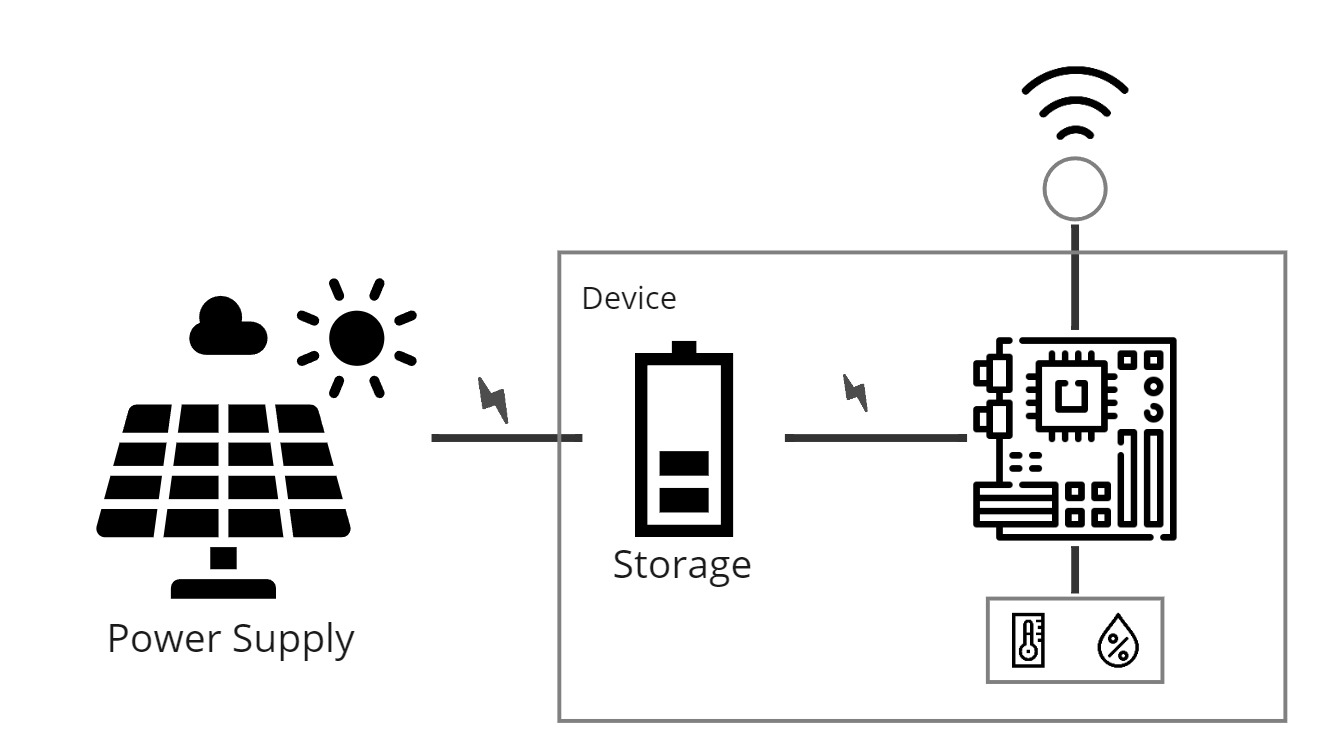
\includegraphics[width=0.75\linewidth]{Imagens/cap6/cap6dinamica.jpg} 
		
	Fonte: elaborado pelo autor.
\end{figure}


Portanto, acontecendo disponibilidade energética, cabe ao dispositivo armazena-la durante um ciclo a medida que os valores vão sendo apresentados ao node. Uma vez cumprido esta etapa, os valores são disponibilizados na forma de recurso que deverá ser dispendido a medida que realiza as atividades solicitadas.

Por fim, o node deverá em todo seu ciclo de vida atuar dinamicamente em conformidade com os modo de operação que represente os valores de recursos energéticos que possui. No experimento estão cobertos quatro modos de atuação a depender das capacidades energéticas:

\begin{enumerate}	
\item Modo Abundante: O Modo Abundante representa o dispositivo que possui recursos energéticos amplamente disponíveis, permitindo o funcionamento completo e otimizado de todas as suas funcionalidades. Aqui, o node atenderá quaisquer solicitação enviada, sem atuação do mecanismo limitante, aproveitando ao máximo a disponibilidade de energia;
\item Modo Atenção: Uma vez atingido este patamar, o node recusar-se a atender algumas solicitações com a motivação de preservar parte dos recursos até que um novo cenário energético seja apresentado;
\item Modo Alerta: O Modo Crítico é alcançado quando o dispositivo está operando com recursos energéticos extremamente limitados, mas ainda tem capacidade para atender algumas solicitações (conforme privilégios ou criticidade das operações). Este modo foi projetado para prolongar a funcionalidade básica do dispositivo enquanto tenta evitar a entrada no Modo Hibernação. 
\item Modo Hibernação: Este modo é ativado quando o dispositivo não possui mais recursos energéticos suficientes para continuar atendendo qualquer solicitação. O dispositivo entra em um estado de hibernação ou equivalente até que recursos energéticos sejam recuperados. Portanto, caso consuma toda sua reserva, o dispositivo estará esgotado energeticamente.
\end{enumerate}

Um modo de operação representa como o mecanismo de \textit{throttling} agirá em detrimento do valor disposto em sua reserva energética, assim contribui para reduzir o uso de recursos, amortizando ou interrompendo o uso energético nos serviços ofertados no node a medida que limita à capacidade de atendimento as solicitações. Naturalmente, estes modos de operação podem sofrer variação, cabe a análise de especificidade e natureza que se destina cada implementação, para isto, a analise desses fatores repousa classe Meios, encontrada na Subseção \ref{cap4:atuacao_meios}. Com isso, os modos de operação guiam a mudança de estados do dispositivo, uma vez que justificados por tal modo, reduz a quantidade de solicitações atendidas, proporcionando maiores momentos em um perfil de inatividade ou equivalente que indique um uso reduzido de recursos. De maneira geral, a dinâmica dos estados do node pode ser visualizada na Figura \ref{fig:cap6maquinaestados}. Por fim, os estados possíveis para o dispositivo são descritos como:

\begin{itemize}
	\item Estado Inativo: Aqui o node estará consumindo a menor quantidade de recurso energético possível. Um node inativo se encontra ocioso, sem realizar nenhuma tarefa enquanto aguarda novas solicitações ou caso necessário, aguarde nova entrada energética disponível.
	\item Estado Ativo: Um node é considerado ativo enquanto executa solicitações. Nesse estado o node utilizará os recursos energéticos necessários para realização das atividades mediante o consumo de seus recursos energéticos. 
	\item Estado Desligado: No experimento, o estado desligado é a indicação que o node não tem mais capacidade de assumir qualquer outro estado enquanto não receber recursos energéticos particularmente em decorrência do esgotamento de suas reservas. Portanto, neste estado, um node não realizará qualquer atividade.	
	
\end{itemize}




\begin{figure}[H]
	\centering
	
	\caption{Maquina de estados do Node.}
	\label{fig:cap6maquinaestados}
	\noindent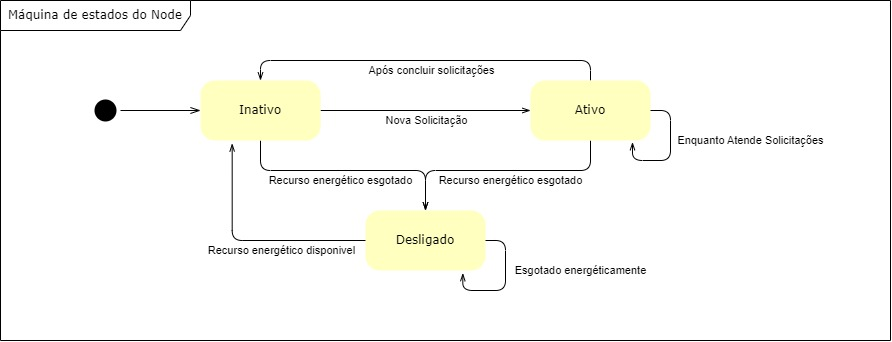
\includegraphics[width=0.75\linewidth]{Imagens/cap6/cap6maquinaestados.jpg} 
	
	Fonte: elaborado pelo autor.
\end{figure}


\section{Definição da variáveis independentes e Dispositivos.}

A teoria de coleta de energia baseia-se na utilização de fontes energéticas disponíveis no ambiente para suprir, parcial ou totalmente, a demanda de um dispositivo inserido neste ambiente. Para o experimento, não há, a princípio, a intenção de analisar as particularidades para cada fonte energética, sua natureza e características de uso ou eficiência. 

Com isso, foi necessário para examinação e avaliação da aderência ao mecanismo de \textit{throttling} proposto abstração de fonte energética, uma vez que os recursos energéticos não seriam provenientes da dinâmica das condições de uma fonte qualquer. Quanto as possíveis novas implementações, ainda sim, caberá os ajustes necessários para atuação do \textit{throttling},  a depender da especificidade das condições submetidas ao node, assim como apresentado em \ref{cap:cap4} na classe Observáveis, esses aspectos são descritos como as questões relativas à entrada energética. 

Todavia, para a execução do experimento é necessário a compreensão sobre à disponibilidade e termos quantitativos de uma fonte de energia que represente valores de entrada para a coleta energética e assim utilizar esses dados como entrada para uma variável independente numérica. Sob tais restrições, os valores utilizados são semelhantes ao comportamento observado por um fonte de energia solar, para isto, seus valores foram concebidos com o auxilio dos dados disponibilizados no Atlas Brasileiro de Energia Solar \cite{martins2017atlas}. Particularmente, a definição dos valores de energia disponível orienta-se pelos parâmetros disponibilizados e apresentados para cidade de Natal/RN, nos termos da média diária de irradiação solar no decorrer  dos meses, o que rotulou-se uma Jornada $J_i$ (para $i = 1,2,...,12$). Os valores são expressos em  $Wh$ , já abstraído a conversão para os termos de consumo conforme Tabela \ref{table:cap6distribuicaonatal} onde cada valor representa o montante energético disponibilizado em uma respectiva jornada.

\begingroup

\setlength{\tabcolsep}{10pt} % Default value: 6pt
\renewcommand{\arraystretch}{1.5} % Default value: 1

\begin{table}[h]
	
	\centering
	\caption{Valor disponibilizado por entrada}
	\smaller[8]
	\tabcolsep=0.05cm
\begin{tabular}{ c l | *{13}{c} }
	\toprule
	Jornada & $Wh$ & \multicolumn{13}{c}{Disponibilizado no Ciclo (c)}\\\cline{3-15}
	& & \begin{tabular}{@{}c@{}} c05 \\(0.007)\end{tabular} &
	\begin{tabular}{@{}c@{}} c06 \\(0.02) \end{tabular}	& 
	\begin{tabular}{@{}c@{}} c07 \\(0.053)\end{tabular} &
	\begin{tabular}{@{}c@{}} c08 \\(0.087) \end{tabular}&
	\begin{tabular}{@{}c@{}} c09 \\(0.105) \end{tabular}&
	\begin{tabular}{@{}c@{}} c10 \\(0.127) \end{tabular}& 
	\begin{tabular}{@{}c@{}} c11 \\(0.136) \end{tabular}& 
	\begin{tabular}{@{}c@{}} c12 \\(0.125) \end{tabular}& 
	\begin{tabular}{@{}c@{}} c13 \\(0.12) \end{tabular}& 
	\begin{tabular}{@{}c@{}} c14 \\(0.101) \end{tabular}& 
	\begin{tabular}{@{}c@{}} c15 \\(0.074)\end{tabular}& 
	\begin{tabular}{@{}c@{}} c16 \\(0.04)\end{tabular}&
	\begin{tabular}{@{}c@{}} c17 \\(0.005)\end{tabular}\\
	
	\hline
	J01 & 5674 & 39.72 & 113.48 & 300.72 & 493.64 & 595.77 & 720.6 & 771.66 & 709.25 & 680.88 & 573.07 & 419.88 & 226.96 & 28.37\\
	\hline
	J02 & 6017 & 42.12 & 120.34 & 318.9 & 523.48 & 631.78 & 764.16 & 818.31 & 752.12 & 722.04 & 607.72 & 445.26 & 240.68 & 30.09 \\
	\hline
	J03 & 6032 &  42.22 & 120.64 & 319.7 & 524.78 & 633.36 & 766.06 & 820.35 & 754.0 & 723.84 & 609.23 & 446.37 & 241.28 & 30.16 \\
	\hline
	J04 & 6082 & 42.57 & 121.64 & 322.35 & 529.13 & 638.61 & 772.41 & 827.15 & 760.25 & 729.84 & 614.28 & 450.07 & 243.28 & 30.41 \\
	\hline
	J05 & 5561 & 38.93 & 111.22 & 294.73 & 483.81 & 583.9 & 706.25 & 756.3 & 695.12 & 667.32 & 561.66 & 411.51 & 222.44 & 27.8\\
	\hline
	J06 & 5075 & 35.52 & 101.5 & 268.97 & 441.52 & 532.88 & 644.52 & 690.2 & 634.38 & 609.0 & 512.58 & 375.55 & 203.0 & 25.38 \\
	\hline
	J07 & 4658 & 32.61 & 93.16 & 246.87 & 405.25 & 489.09 & 591.57 & 633.49 & 582.25 & 558.96 & 470.46 & 344.69 & 186.32 & 23.29 \\
	\hline
	J08 & 4773 & 33.41 & 95.46 & 252.97 & 415.25 & 501.16 & 606.17 & 649.13 & 596.62 & 572.76 & 482.07 & 353.2 & 190.92 & 23.87\\
	\hline
	J09 & 5571 & 39.0 & 111.42 & 295.26 & 484.68 & 584.95 & 707.52 & 757.66 & 696.38 & 668.52 & 562.67 & 412.25 & 222.84 & 27.86\\
	\hline
	J10 & 5971 & 41.8 & 119.42 & 316.46 & 519.48 & 626.95 & 758.32 & 812.06 & 746.38 & 716.52 & 603.07 & 441.85 & 238.84 & 29.86 \\
	\hline
	J11 & 6112 & 42.78 & 122.24 & 323.94 & 531.74 & 641.76 & 776.22 & 831.23 & 764.0 & 733.44 & 617.31 & 452.29 & 244.48 & 30.56 \\
	\hline
	J12 & 6269 & 43.88 & 125.38 & 332.26 & 545.4 & 658.25 & 796.16 & 852.58 & 783.62 & 752.28 & 633.17 & 463.91 & 250.76 & 31.35 \\
\bottomrule
\end{tabular}
\label{table:cap6distribuicaonatal}
\\
\footnotesize Fonte: adaptado de \citeauthor{martins2017atlas}, (\citeyear{martins2017atlas})

\end{table}
\endgroup

O fator de distribuição atribuído a cada ciclo representa o fator da incidência solar em um dado instante em relação ao total disponível em uma jornada num intervalo de 24 ciclos. Para atribuição dos pesos dispostos em cada ciclo, foi utilizada a referencia disponibilizada em \citeonline{tutiempo2023} para o dia 12 de dezembro de 2023. Aqui cabe destacar que a limitação de adotar a distribuição solar para um dia especifico é justificada pela intenção de apenas conceber os valores capazes de cobrir o propósito do experimento, a medida que paralelamente aproxima-se dos termos característicos de  uma fonte energética solar. Assim, obteve-se a definição dos valores ofertados, com a determinação valores atribuídos em referencia as jornadas aplicados aos fatores de incidência encontrados em cada intervalo (ciclo). Particularmente, os ciclos $c_0, c_1,... c_4$ e $c_{18}, c_{19},... c_{23}$ possuem peso atribuído zero, pois representam ciclos onde não existe energia coletável significante, em conformidade com a referencia solar e suas características utilizada.

Os valores de cada ciclo são ofertados como estimulo ao node provedor no decorrer do experimento, e ao fim do ciclo 23 de uma dada jornada, inicia-se a jornada seguinte até que todos os 24 ciclos das 12 jornadas sejam ofertadas. Esta abordagem garante que todos os cenários previstos para o experimento foram cobertos em sua execução e seus resultados analisados na Seção \ref{cap6:avaliacao}.

\subsection{Dispositivos}

Foi construído um modelo capaz de representar um dispositivo sensor embarcado com os mecanismos do \textit{throttling}, este node é uma abstração que deverá receber estímulos como entradas energéticas em um cenário simulado, a medida que utiliza esses recursos para atender solicitações continuas em uam interface de acesso provisionada. A visão geral do node provedor e componentes pode ser visto na Figura \ref{fig:cap6providernode}. Além disso, o código fonte do mesmo está disponível no repositório Git\footnote{Código-Fonte do Node Provedor em \url{https://github.com/eusoupaulolopes/mst_experiments}.}  para análise e colaboração.

\begin{figure}[H]
	\centering
	
	\caption{Componentes do Node Provedor.}
	\label{fig:cap6providernode}
	\noindent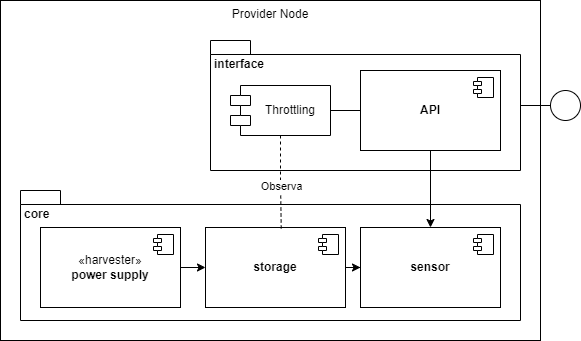
\includegraphics[width=0.75\linewidth]{Imagens/cap6/cap6providernode.png} 
	
	Fonte: elaborado pelo autor.
\end{figure}

Os elementos idealizados que constituem o node provedor são referentes aos seguintes componentes:

\textbf{\textit{Power Supply}}, é responsável por fornecer a energia necessária para o funcionamento do dispositivo, simulando a coleta de energia de acordo com os ciclos descritos na Tabela \ref{table:cap6distribuicaonatal}. O componente atuará em paralelo a outras atividades realizadas. Caso o armazenamento do dispositivo esteja completamente cheio, ainda assim os valores de entrada serão entregues, representando desperdício energético. O esgotamento energético do dispositivo não representa a incapacidade de receber novas entradas energéticas e com isso, assumir novos estados de operação.  

\textbf{\textit{Storage}}, responsável por armazenar os valores energéticos oferecidos mediante sua capacidade e a partir disso, oferecer a energia coletada, sendo um componente suplementar com o objetivo de manter disponibilidade energética do dispositivo sob certas circunstancias. A capacidade definida para o \textit{Storage} do node provedor pode ser ajustada e deve representar a aderência da configuração proposta para um \textit{buffer} energético no cenário de uso.  

\textbf{\textit{Sensor}}, cabe a este componente simular as atividades executadas pelo dispositivo. Dentre as características presentes em Sensor, esta a indicação do gasto energético momentâneo mediante o estado que se encontra em referencia aos possíveis estados já apresentados na Figura \ref{fig:cap6maquinaestados}. Assim, é possível configurar um node para embarcar um ou mais sensores, mediante implementação da especificação de seus custos energéticos operacionais em cada estado possível. Assim, o dispositivo é capaz de simular um ou mais sensores diversos, temperatura, umidade, pressão, luminosidade, presença, entre outros, caso necessário.

\textbf{\textit{Interface}} é o ponto de entrada para recebimento das solicitações de sensoriamento, componente de interação com o dispositivo. O mecanismo de \textit{throttling} atuará acoplado a interface provida, controlando a vazão de atendimento a medida que permite ou bloqueia as requisições recebidas em garantia de manter o modo de operação em sincronismo ao estado das suas capacidades energéticas. Assim, uma vez atingido um limiar observado, instantaneamente o dispositivo poderá negar novas requisições ainda na interface, impedindo assim a propagação da mensagem que estimularia o seu grupo de sensores para atender a demanda solicitada, e através disso amortizando o gasto energético total do node.




\section{Instrumentalização.}
\label{cap6:instrumentalizacao}
Para garantir a precisão e a confiabilidade dos dados coletados no experimento, alguns instrumentos de medição foram utilizados escolhido com base em sua adequação às necessidades específicas do experimento. 

A coleta de dados foi realizada em intervalos regulares de 10 segundos definidos no plano experimental. Dada também a necessidade de armazenamento dos dados capturados, optou-se pelo sistema de coleta e monitoramento encontrado na solução Prometheus\footnote{Disponível em \url{https://prometheus.io/}.}, capaz de entregar os dados de maneira estruturada em um formato que facilita acompanhar a execução do experimento através dos logs gerados bem como análise futura do resultados. 

Para tanto, de maneira transparente é embarcado no dispositivo um cliente Prometheus \textit{Exporter} com a capacidade de expor os dados observáveis e de interesse periodicamente a um agente externo chamado \textit{Collector}. Durante atividade de coleta, cabe ao agente coletor as ações de solicitar os dados providos no cliente e também armazenar os dados na forma de séries temporais em um modelo que permite consultas em um formato especifico chamado PromQL - \textit{Prometheus Query Language} e com isso possibilitando a visualização dos dados em gráficos customizáveis ou a criação de alertas, caso necessário.

Todos os dados recuperados pelo coletor são disponibilizados e mantidos no Prometheus. A Figura \ref{fig:cap6instrumentalizacao} ilustra a dinâmica entre node e agente externo coletor e por sua vez a disponibilidade dos dados para uma \textit{dashboard}. 

\begin{figure}[H]
	\centering
	
	\caption{Componentes do Node Provedor.}
	\label{fig:cap6instrumentalizacao}
	\noindent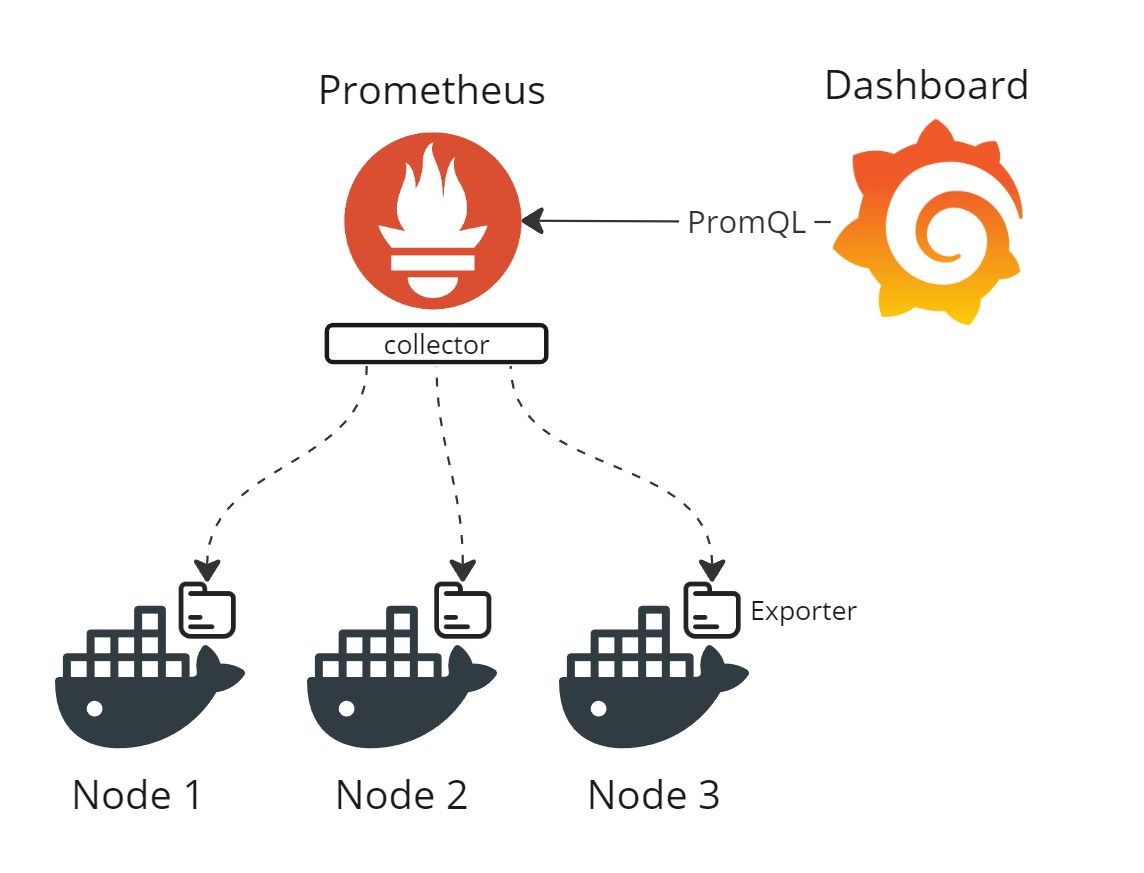
\includegraphics[width=0.75\linewidth]{Imagens/cap6/cap6instrumentalizacao.jpg} 
	
	Fonte: elaborado pelo autor.
\end{figure}

A concepção do quadro - \textit{dashboard} para visualização dos dados é destinado para realizar consultas sobre os valores coletados ou acompanhar o comportamento dos nodes provedores ainda em tempo de execução do experimento, a Figura \ref{fig:cap6bashboard} apresenta o aspecto da interface de acesso.

\begin{figure}[H]
	\centering
	
	\caption{Dashboard para visualização dos resultados.}
	\label{fig:cap6bashboard}
	\noindent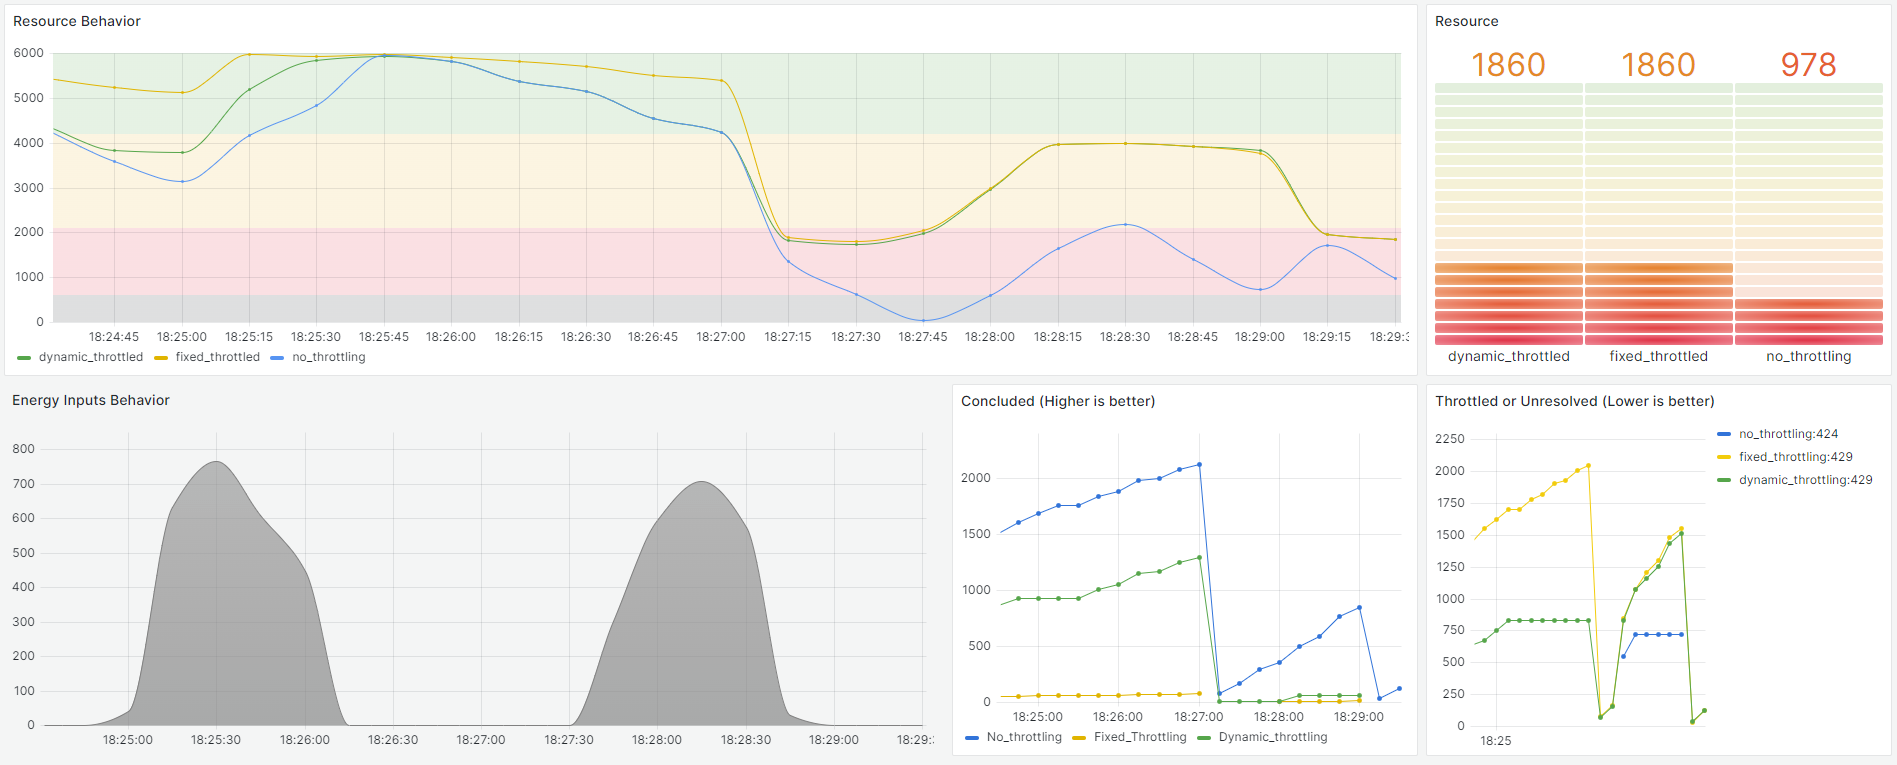
\includegraphics[width=1\linewidth]{Imagens/cap6/cap6dashboard.png} 
	
	Fonte: elaborado pelo autor.
\end{figure}

Vale destacar que o processo de instrumentalização não exerce influencia sobre a capacidade energética do node. Seu uso e custos são transparentes para a implementação em si, funcionando como um agente independente que não interfere nas dinâmicas energéticas colocadas em análise.


\section{Execução.}
\label{cap6:execucao}
\section{Avaliação.}
\label{cap6:avaliacao}
 